\subsection{Matriz de Transição}

Dado $N \geq 2$, dizemos que $A$ é uma matriz de transição se $A = (a_{ij})_{1 \leq i,j \leq N}$ é uma matriz quadrada de ordem $N$ tal que $a_{ij} \in \lbrace 0, 1 \rbrace$ para todo $1 \leq i,j \leq N$.
Se $A$ é uma matriz de transição, definimos o conjunto $\Sigma_A$ por
$$\Sigma_A = \lbrace (x_0 \, x_1 \, x_2 \, \dots) \in \Sigma_N : a_{x_k x_{k+1}} = 1 \text{ para todo } k \geq 0 \rbrace.$$
Observe que se $x \in \Sigma_A$, então $\sigma(x) \in \Sigma_A$.
Desse modo, podemos definir a função $\sigma_A: \Sigma_A \to \Sigma_A$ como sendo a restrição de $\sigma$ em $\Sigma_A$.

Vamos estudar a dinâmica da família quadrática para $\mu = 3.839$.
Se $a = 0.149888$, $\varepsilon = 10^{-3}$ e $I = (a - \varepsilon, a + \varepsilon)$, então é possível mostrar que $h^3(I) \subset I$ e $|D h^3(I)| < 1$ e, portanto, o intervalo $I$ possui um ponto periódico atrator de $h$ de período primo $3$. Se $a_1$, $a_2$ e $a_3$ são os elementos dessa órbita em ordem crescente, então
$$a_1 \simeq 0.149888, \quad a_2 \simeq 0.489149 \quad \text{ e } \quad a_3 \simeq 0.959299.$$

Com auxílio do Teorema de Sharkovsky e do Teorema de Singer, que estudaremos na sequência, podemos concluir que $h$ possui infinitos pontos periódicos e essa é a única órbita atratora de $h$.

\begin{figure}[!htb]
\centering
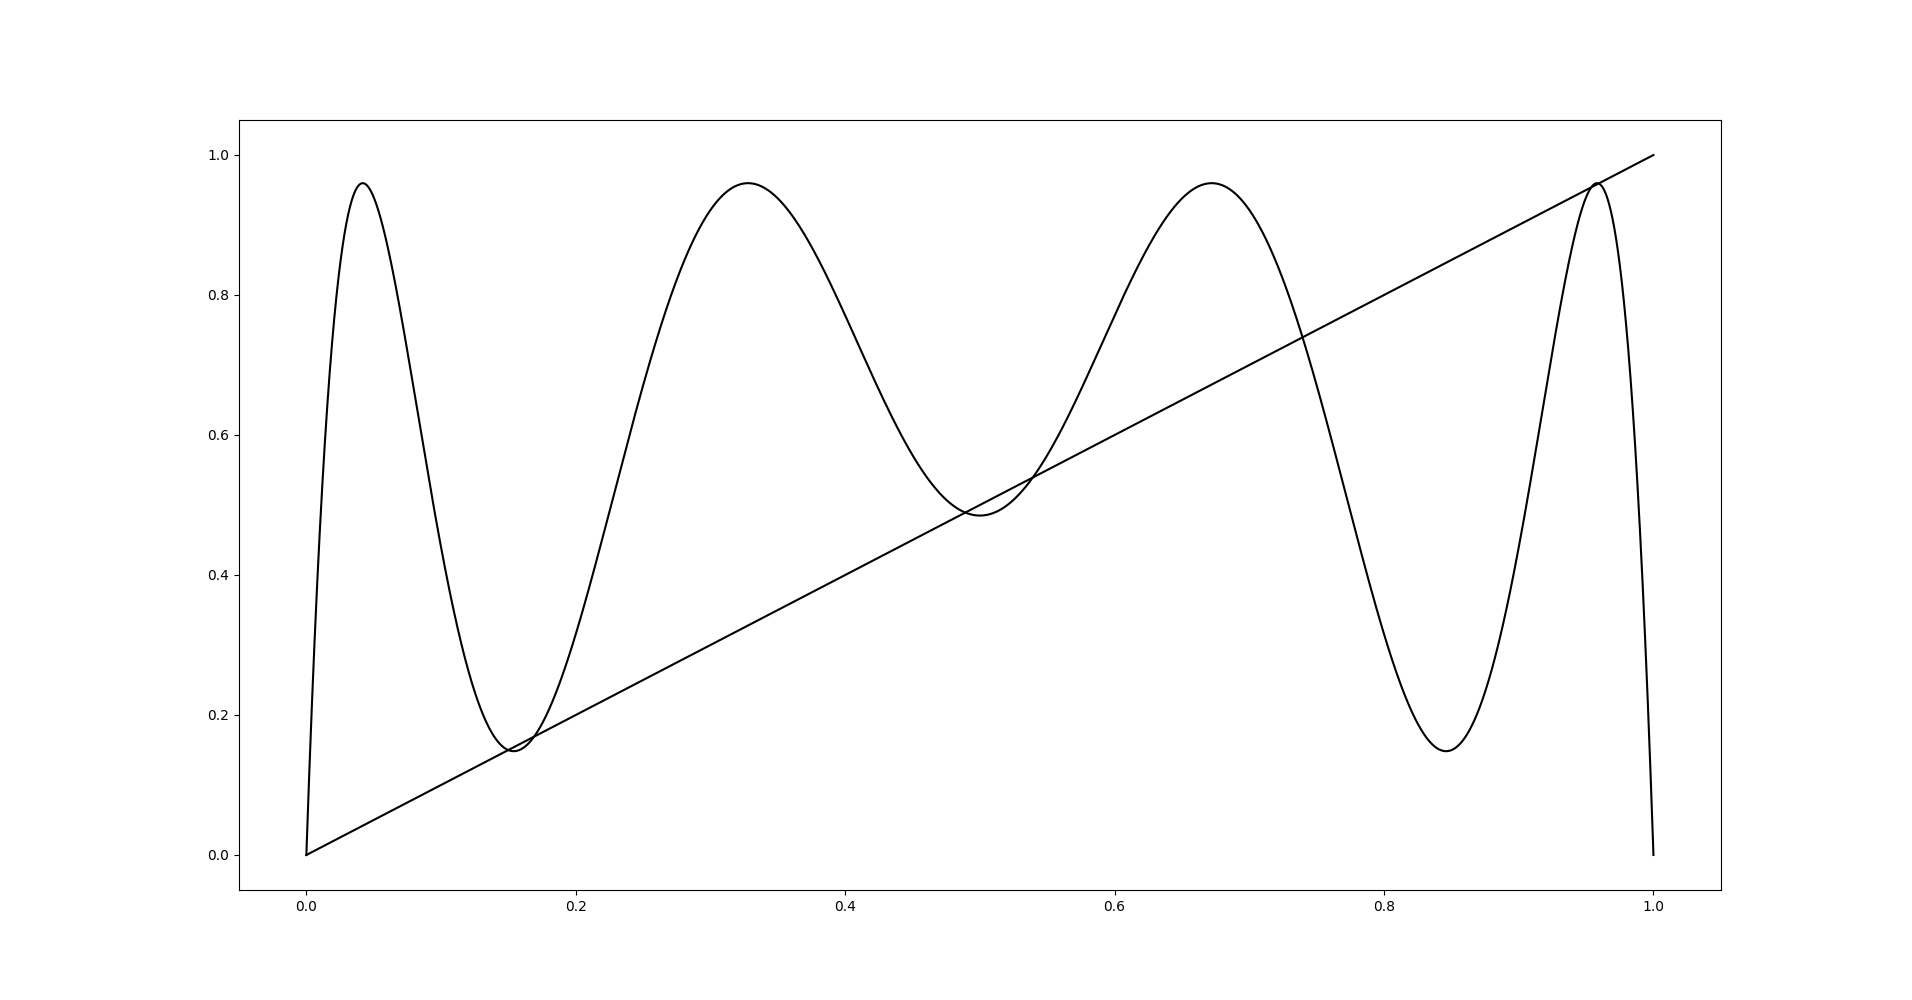
\includegraphics[scale=0.6]{images/h_3,839.png}
\caption{Gráfico de $h^3$ para $\mu = 3.839$.}
\label{h_3,839}
\end{figure}

De modo análogo, concluímos que $h$ possui outra órbita de tamanho $3$. Se $b_1$, $b_2$ e $b_3$ são os elementos dessa órbita em ordem crescente, então
$$b_1 \simeq 0.169040, \quad b_2 \simeq 0.539247 \quad  \text{ e } \quad b_3 \simeq 0.953837.$$

Observando o gráfico de $h^3$, vemos que para cada $b_i$, existe $b'_i$ no lado oposto de $b_i$ em relação ao ponto $a_i$ tal que $h^3(b'_i) = b_i$. Defina $A_1 = (b'_1, b_1)$, $A_2 = (b'_2, b_2)$ e $A_3 = (b_3, b'_3)$.

\begin{figure}[!htb]
\centering
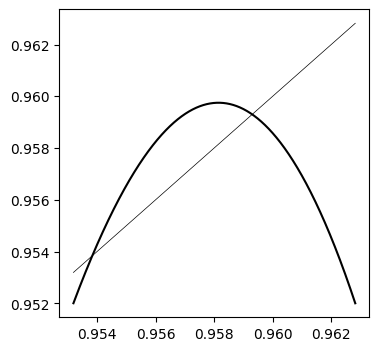
\includegraphics[scale=0.6]{images/h_3,839(a_3).png}
\caption{Gráfico de $h^3$ numa vizinhança de $a_3$ para $\mu = 3.839$.}
\label{h_3,839(a_3)}
\end{figure}

Sendo $h^3$ simétrica em relação ao ponto $\frac{1}{2}$, temos que $h(b'_2) = h(b_2) = b_3$.
Além disso, podemos observar que $h(b'_1) = b'_2$ e $h(b'_3) = b'_1$ e, portanto, $h$ mapeia de forma monótona $A_1$ em $A_2$ e $A_3$ em $A_1$. Observando que o máximo de $h$ em $A_2$ é $h( \frac{1}{2}) = 0.95975 < b'_3$, concluímos que $h(A_2) \subset A_3$.

Sabemos que se $x \notin [0, 1]$, então $\lim_{n \to \infty} h^n(x) = -\infty$.
Além disso, o único ponto periódico em $A_i$ é $a_i$ e todos os pontos em $A_i$ tendem para a órbita de $a_i$.
Desse modo, todos os outros pontos periódicos de $h$ residem no complemento de $A_1 \cup A_2 \cup A_3$ em $[0, 1]$, que é formado por quatro intervalos fechados. Sejam $I_0 = [0, b'_1]$, $I_1 = [b_1, b'_2]$, $I_2 = [b_2, b_3]$ e $I_3 = [b'_3, 1]$ tais intervalos.

\begin{proposition}
Se $x \notin \lbrace 0, a_1, a_2, a_3 \rbrace$ é um ponto periódico de $h$, então $x \in I_1 \cup I_2$.
\end{proposition}

\begin{proof}
Observando que $h$ é monótona em cada $I_k$, temos que $h(I_0) = I_0 \cup A_1 \cup I_1$, $h(I_1) = I_2$, $h(I_2) = I_1 \cup A_2 \cup I_2$ e $h(I_3) = I_0$. Desse modo, se $x \in I_1 \cup I_2$ é periódico, então órbita de $x$ está contida em $I_1 \cup I_2$.

Por outro lado, se $x \in I_0 \backslash \lbrace 0 \rbrace$, existe um menor $n \geq 1$ tal que $h^n(x) \notin I_0$. Se $h^n(x) \in A_1$, então $x$ não pode ser periódico, pois o único ponto periódico de $A_1$ é $a_1$.
Se $h^n(x) \in I_1$, então $x$ não pode ser periódico, pois caso contrário a órbita de $x$ estaria contida em $I_1 \cup I_2$ e nunca retornaria para $I_0$.
Finalmente, se $x \in I_3$, então $h(x) \in I_0$ e a análise é análoga.
\end{proof}

Considere o conjunto $\Lambda = \lbrace x \in I_1 \cup I_2 : h^n(x) \in I_1 \cup I_2 \text{ para todo } n \geq 1 \rbrace$.
Pela proposição anterior, todos os pontos periódicos de $h$ estão em $\Lambda$, com exceção dos pontos $0$, $a_1$, $a_2$ e $a_3$.

Para a demonstração do próximo teorema, vamos considerar a matriz de transição
$$A =
\begin{pmatrix}
0 & 1 \\
1 & 1 \\
\end{pmatrix}.$$
Seja $S: \Lambda \to \Sigma_A$ a função dada por $S(x) = (x_0 \, x_1 \, x_2 \, \dots)$, onde $x_k = 1$ se $h^k(x) \in I_1$ e $x_k = 2$ se $h^k(x) \in I_2$ para todo $k \geq 0$. Observe que $S$ está bem definida, pois $h(I_1) = I_2$ e $h(I_2) \subset I_1 \cup I_2$ e, portanto, $a_{x_k x_{k+1}} = 1$ para todo $k \geq 0$. 


\begin{lemma}
Existe $n_0 \geq 1$ tal que $|D h^n(\Lambda)| > 1$ para todo $n \geq n_0$.
\end{lemma}

\begin{proof}
Inicialmente, podemos observar graficamente que $|D h(I_1 \cup I_2)| \geq \nu$ para algum $\nu \in (0, 1)$.
Podemos observar também que o subconjunto de $I_1 \cup I_2$ no qual a derivada em módulo de $h^3$ é menor que ou igual à $1$ é formado por três intervalos fechados e que cada um desses intervalos possui intersecção vazia com $\Lambda$ e, portanto, $|D h^3(\Lambda)| \geq \lambda$ para algum $\lambda > 1$.

Por fim, sejam $x \in \Lambda$ e $K \geq 1$ tal que $\nu^2 \lambda^K > 1$. Se $n_0 = 3K$ e $n \geq n_0$, podemos escrever $n = 3L + m$, onde $L \geq K$ e $0 \leq m \leq 2$. Desse modo, se $m = 0$, então $ |D h^n(x)| = |D h^{3L}(x)|
\geq \lambda^L > 1$; se $m = 1$, então $|D h^n(x)| = |D h(h^{3L}(x))| |D h^{3L}(x)| \geq \nu \lambda^L > 1$; e se $m = 2$, então $|D h^n(x)| = |D h(h^{3L+1}(x))| |D h(h^{3L}(x))| |D h^{3L}(x)| \geq \nu^2 \lambda^L > 1$.
\end{proof}

Com isso, enunciamos o teorema cuja demonstração é análoga à do Teorema \ref{teo 6-1}.

\begin{theorem}
$h|_\Lambda$ e $\sigma_A$ são topologicamente conjugadas por $S$.
\end{theorem}

\begin{proof}
Exercício.
\end{proof}

Sabendo que $h|_\Lambda$ e $\sigma_A$ são topologicamente conjugadas, a proposição a seguir nos permite saber a quantidade de pontos periódicos de $h|_\Lambda$ de período $n$ para todo $n \geq 1$.

\begin{proposition}
Se $A$ uma matriz de transição de ordem $N$, então $\sigma_A$ possui $\tr(A^n)$ pontos periódicos de período $n$ para todo $n \geq 1$.
\end{proposition}


\begin{proof}
Inicialmente, observe que se $(x_0 \, x_1 \, x_2 \, \dots) \in \Sigma_N$ é um ponto periódico de $\sigma$ de período $n$, então $x_k = x_{k+n}$ para todo $k \geq 0$.
Desse modo, $(x_0 \, x_1 \, x_2 \, \dots) \in \Sigma_A$ se, e somente se, $a_{x_0 x_1} = a_{x_1 x_2} = \cdots = a_{x_{n-1} x_0} = 1$ e, portanto, a quantidade de pontos periódicos de $\sigma_A$ de período $n$ é dada por
$$\sum_{1 \leq x_0, \dots, x_{n-1} \leq N} a_{x_0 x_1} a_{x_1 x_2}  \dots a_{x_{n-1} x_0}.$$
Por outro lado, é imediato verificar que essa soma é $\tr(A^n)$.
\end{proof}
